\begin{figure*}[h]                                                           
 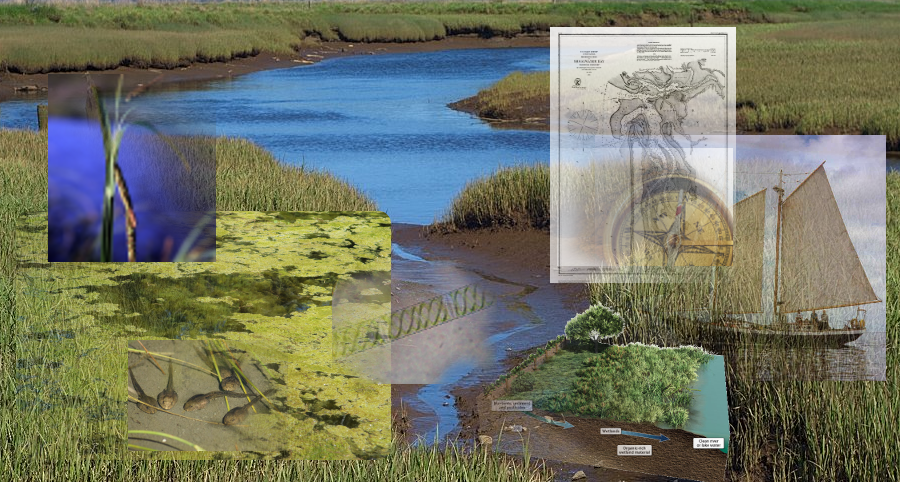
\includegraphics[width=\linewidth]{./media/images/multiple_paths}%
  \scriptsize{\textsc{\\gps enabled interactive fiction} lets your readers explore
  multiple disciplines for a given location including biology, history,
  wildlife, and conservation.}
  \label{fig:multiple_paths}%                                                 
\end{figure*}                                                                
\begin{quotation} 
\noindent\color{Sepia}{{\textit{\textbf{“You never know what's around the corner. It could be everything. Or it could be nothing. You keep putting one foot in front of the other, and then one day you look back and you've climbed a mountain.”}}}}\\[.5mm]
%remove following line space if you're tight on vertical room and need to fit on
%single page

\hfill\color{Sepia}{\small{\textendash \textsc{Tom Hiddleston}}}
\end{quotation} 
\begin{figure*}[h]                                                           
 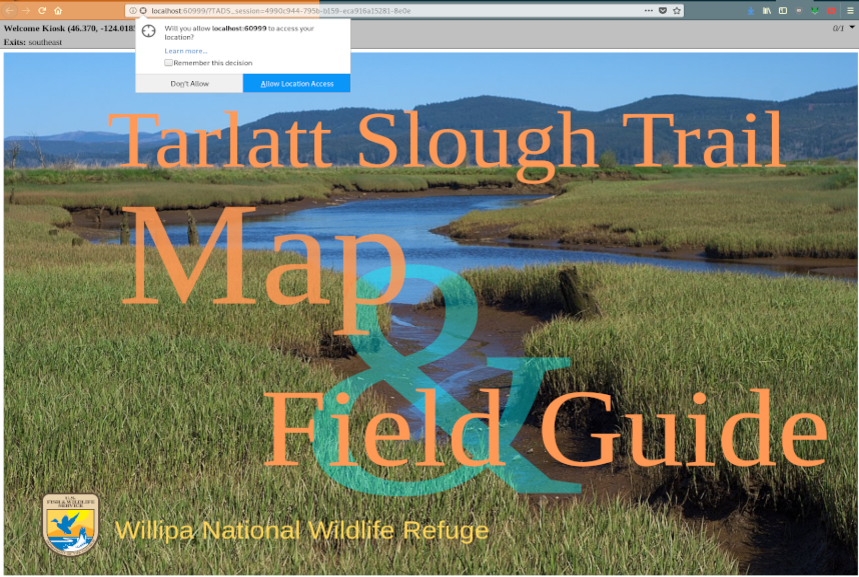
\includegraphics[width=\linewidth]{./media/images/trail_gps.pdf}%
  \scriptsize{\textsc{\\ The user is presented} with a dialog asking for
    permission to access the user's \textsc{gps} device and current location.}
  \label{fig:gps_location}%                                                 
\end{figure*}
This tutorial outlines the build process for creating \textsc{gps} enabled
Interactive fiction. It uses the \textsc{tads3} build system with Javascript
hooks to report \textsc{gps} coordinates from the client's browser to the
Interactive Fiction server.
\marginnote{The compressed version of all the files in the project
  \textattachfile{media/gps.zip}{\color{red!50!black}{\emph{gps.zip}}} (if your PDF
  viewer supports it) is attached here to make it convenient for you to get started}
\noindent Part of \textsc{tads3}'s power lies in it's ability to seamlessly
incluse web objects, styling, and Javascript through the user's browser directly into
your Interactive Fiction. We'll leverage this ability to access the user's
\textsc{gps} sensor to update your story based on the user's current location.
\marginnote{We want to make the experience easy for players not experienced with the parser and thus make heavy use of links}[2em]
The Javascript embedded in the \textsc{tads3} system polls the \textsc{gps}
device every five seconds to see if the traveler has come 
within approximately 10 meters of a known location. When the system detects a
user's new programmed location it will (optionally) send an alert and
automatically update the user's display with a description of their new
surroundings.

Exploration may be had by entering text directly into the parser or through
links embedded in the text so that the traveler need only click on a link to
learn more.

\subsection{prerequisites}
\noindent Creating a workable system requires only that you have a working
\textsc{frobtads} installation. These instructions assume a working Linux installation though they may be easily
adapted to either the Macintosh or Windows platforms. The difference between the
Windows and the Linux and Mac platforms lies largely in the latter two's lack of graphical user
interface. Depending on your development style you may consider the
console\textendash based environment a feature.
\marginnote{The \href{http://www.tads.org/tads3.htm}{\textsc{frobtads } download page}
  makes downloading \textsc{frobtads} easy for your platform. The
  \href{https://github.com/realnc/frobtads}{\textsc{frobtads} repository 
    distribution} is also available for compiling \textsc{frobtads} from the
  latest source.}[-8em]

Once you've finished installing \textsc{frobtads} you can test your installation
by executing the \texttt{t3make} command on the command line. If you receive the
command's help message you've correctly installed the compiler. You can further
test the \textsc{frob} interpreter by entering the \texttt{frob} command on the
command line; you should be greeted with \textsc{frob}'s help message.
\subsection{install generator-tads}
Generator Tads makes it easier to start new projects as it will automatically
create a complete \textsc{tads3} project after answering a few questions about
your project. The template comes complete with build environments for both the
web and terminal versions of your work of \textsc{if}. \textsc{generator-tads}
requires \textsc{nodejs} and \textsc{yeoman} to work.
\subsection{install Yeoman}
\begin{lstlisting}
sudo npm install -g yo
...
Running sanity checks on your system

✔ Global configuration file is valid
✔ NODE_PATH matches the npm root
✔ Node.js version
✔ No .bowerrc file in home directory
✔ No .yo-rc.json file in home directory
✔ npm version
✔ yo version

Everything looks all right!
+ yo@2.0.5
\end{lstlisting}
\marginnote{\href{https://www.anthonyirwin.com/generator-tads/}{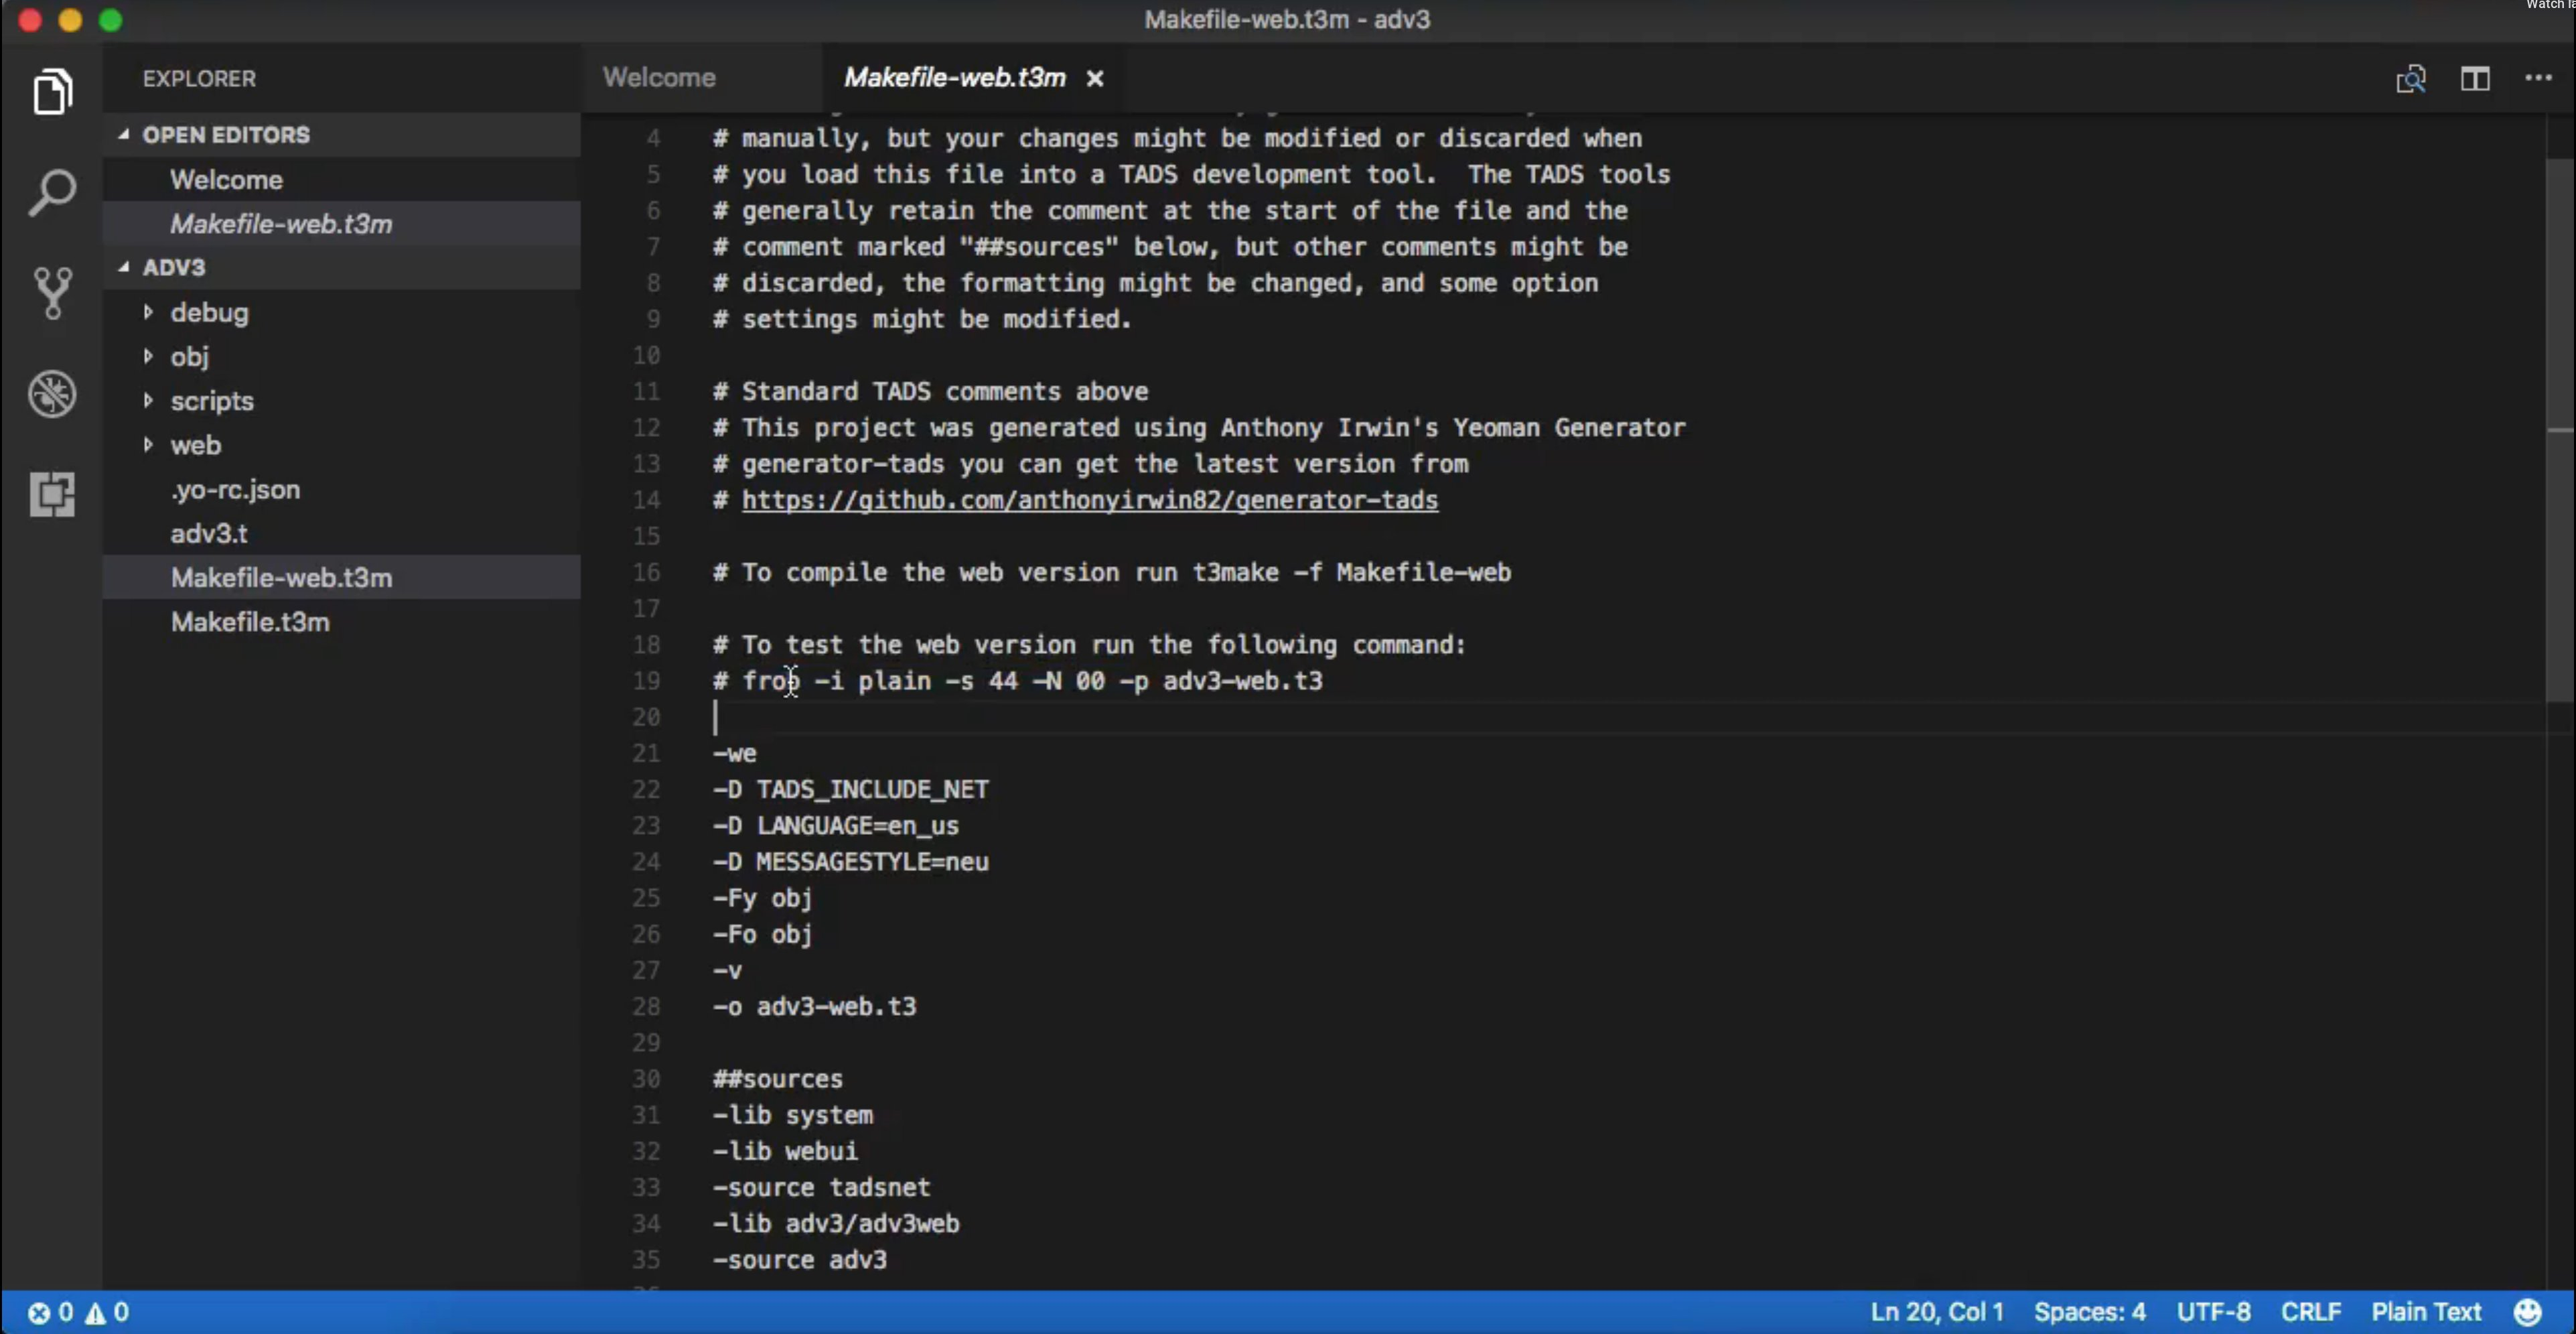
\includegraphics[width=\linewidth]{./media/images/template}\\
  Generator Tads' brief video tutorial makes creating new \textsc{tads3}
  instances easy to learn.}}[-13em]
\subsection{Install Generator Tads using npm}
Notice the \texttt{-g} switch in the \textsc{npm} command. This indicates that we wish to
install \textsc{generator tads} globally but a local instance may be installed
as well.

\begin{lstlisting}
  sudo npm install -g generator-tads
 > spawn-sync@1.0.15 postinstall /usr/lib/node_modules/generator-tads/node_modules/spawn-sync
> node postinstall

+ generator-tads@1.0.2
added 209 packages from 114 contributors in 10.307s
\end{lstlisting}
Create a project directory. This directory may be anywhere you like. I've used
the \texttt{/home/cstevens/doc/gps} directory for this example:

\begin{lstlisting}
  mkdir /home/cstevens/doc/gps
  cd /home/cstevens/doc/gps
\end{lstlisting}
Once you're in the directory, simply run \textsc{yo} to be greeted with a
walkthrough for creating a new project.
\begin{lstlisting}
  yo tads
\end{lstlisting}
If everything worked out alright you will be greeted with this welcome screen
\begin{verbatim}

     _-----_
    |       |    ╭──────────────────────────╮
    |--(o)--|    │ Welcome to the wonderful │
   `---------´   │      tads generator!     │
    ( _´U`_ )    ╰──────────────────────────╯
    /___A___\   /
     |  ~  |
   __'.___.'__
 ´   `  |° ´ Y `

? What type of application do you want to create?
> adv3 Application
  adv3Lite Application
\end{verbatim}
Be certain to select the first option, \texttt{adv3 Application} as the
\textsc{adv3lite} library does not have the features required for embedding web
scripts into your work of \textsc{if}.
NOTE: The project's HTML description cannot contain  at least the ' character.

The system will ask you a few things about your story
\begin{lstlisting}
? What type of application do you want to create? adv3 Application
? Project Name: Cannot contain  / : * ? " < > | or <space> characters. This is the project filename. gps
? Authors Name D. Cooper Stevenson
? Authors Email Address cooper@discdigest.xyz
? The Title of your interactive fiction game GPS Enabled Interactive Fiction
? The Text description of your interactive fiction game Explorers experience the fabric of their surroundings as they may now engage in their environment fully. Your mobile device serves as a gateway to this area's history, biology, wildlife, and archi tecture. Several challenges await, are you ready?
? The HTML description of your interactive fiction game Explorers experience the fabric of their surroundings as they may now engage in their environment fully. Your mobile device serves as a gateway to this areas history, biology, wildlife, and architecture. Several challenges await, are you ready? 
? The IFID for your interactive fiction game. This must be unique for each game the same way as an ISBN is unique for each boo k. You can get an IFID at http://www.tads.org/ifidgen/ifidgen 478AF834-3D02-4B86-9708-88B9572ED8AF   
? The root path to third-party extensions like adv3Lite: Do not add a trailing / E.g. ../extensions ../extensions
   create gps.t
   create Makefile.t3m
   create Makefile-web.t3m
\end{lstlisting}
Let's compile the template
\begin{lstlisting}
t3make
TADS Compiler 3.1.3  Copyright 1999, 2012 Michael J. Roberts
        Files to build: 5
        symbol_export gps.t -> obj/gps.t3s
        compile gps.t -> obj/gps.t3o
        link -> gps.t3p
        preinit -> gps.t3
        add_resources -> gps.t3
        + GameInfo.txt (GameInfo.txt)
\end{lstlisting}
Now we can run the game
\begin{lstlisting}
frob gps
\end{lstlisting}
\begin{figure*}[h]                                                           
 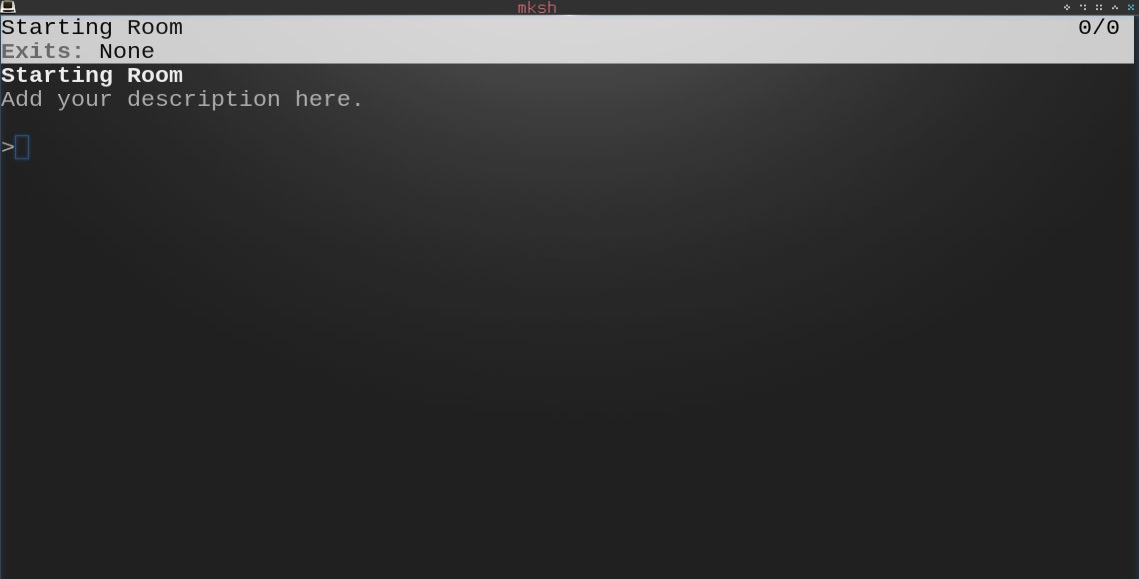
\includegraphics[width=\linewidth]{./media/images/new_text_game.pdf}%
  \scriptsize{\textsc{\\After answering a few questions} about your work of
    Interactive Fiction and compiling  you're greeted with a fresh
    \textsc{tads3} instance running through the \textsc{frob} interpreter.}
  \label{fig:new_text_game}%                                                 
\end{figure*}                                                                
\subsection{compiling a web instance}
\begin{lstlisting}
t3make -f Makefile-web
\end{lstlisting}
Running the instance is simply a matter of running
\begin{lstlisting}
frob -i plain -s 44 -N 00 -p gps-web.t3
\end{lstlisting}
Click on the resulting \textsc{connectwebui} link. A web browser (or new tab)
will appear with your new web\textendash based instance. Let's add some introductory text and a description for the initial area of exploration. The text that follows are excerpts in Chapter 10 of from John L. Stephens' \emph{Incidents of Travel in Yucatan}.
\marginnote{\href{http://www.gutenberg.org/files/33129/33129-h/33129-h.htm}{John L. Stephens' Incidents of Travel in Yucatan}}[-2em]
In \texttt{gps.t} we'll start
with modifying the character set to \textsc{utf-8} (we're civilized people after all) and the \texttt{GameMainDef} function as follows
\begin{lstlisting}
#charset "UTF-8"
...
gameMain: GameMainDef {
    initialPlayerChar = me
    showIntro() {
	"<center><img src='https://web.archive.org/web/20131004041019if_/http://www.gutenberg.org/files/33129/33129-h/images/p165_8.png' width='100%' align='center'></center>
	 <p>
	 <p>";
    }
}
\end{lstlisting}
\begin{figure*}[h]                                                           
 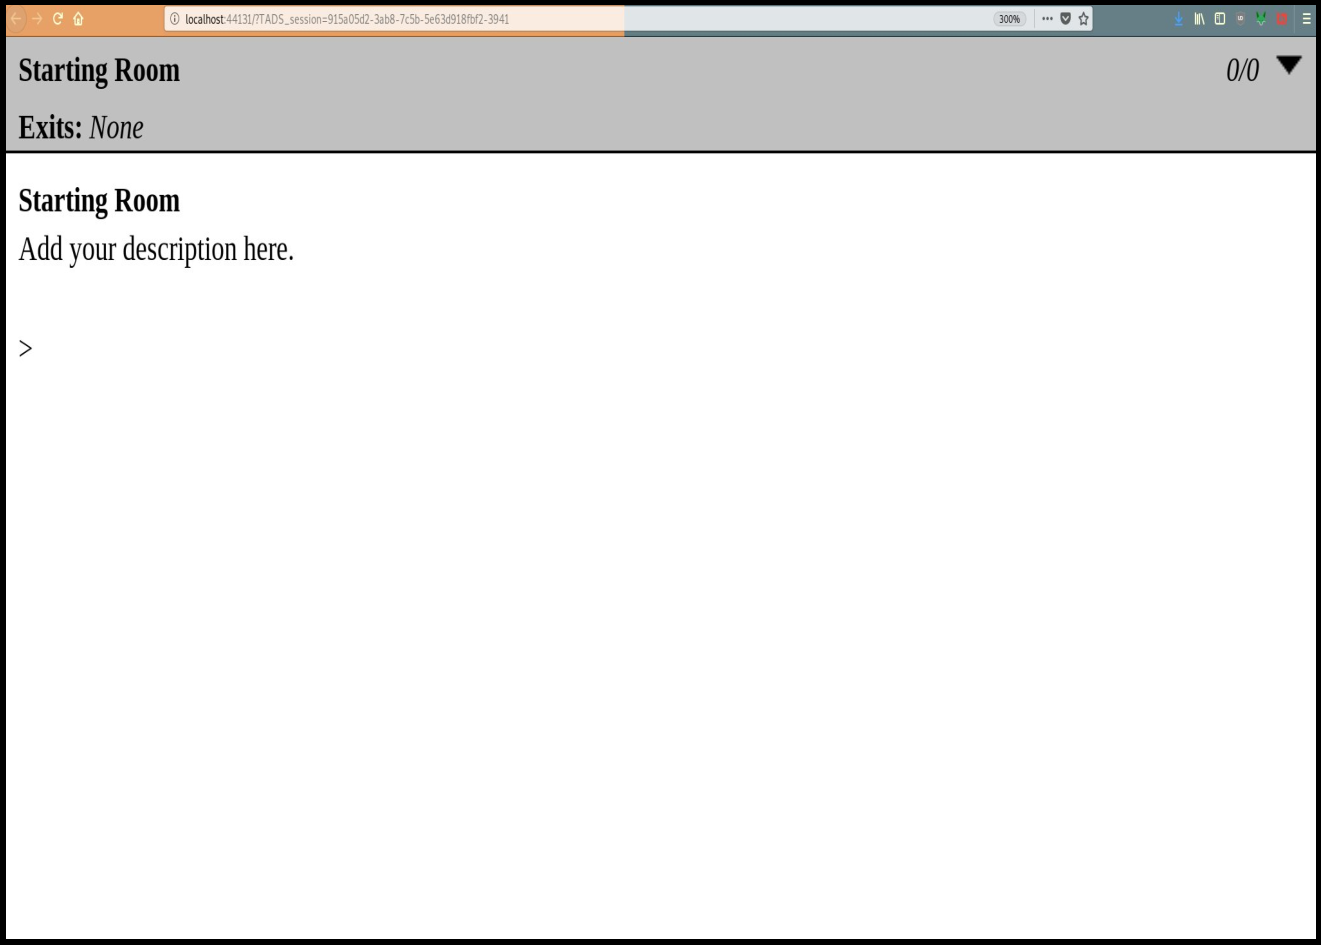
\includegraphics[width=\linewidth]{./media/images/new_web_game.pdf}%
  \scriptsize{\textsc{\\The foundation is now laid } for both a web and
    text\textendash based work of \textsc{if}}
  \label{fig:new_web_game}%                                                 
\end{figure*}
Notice the \texttt{<img src='https://...>} tag in the
\texttt{\scriptsize{showIntro}} function.
\textsc{tads3} allows you to inject \textsc{html, css, and javascript} code
directly into your prose or as a separate library file as we'll see with the
\textsc{gps} process we'll run in the background. If you compile your simulation
for text mode\textemdash handy for concentrating on your writing\textemdash the
compiler will simply ignore these directives and run the
console version. 

Let's add some text to the first area and add an additional area to the
Southeast. First, modify \texttt{gps.t} with an updated room name and a
connection to the Southeast Facade to the Southeast:

\begin{lstlisting}
firstRoom: Room 'Noble Courtyard'
"Among my many causes of regret for the small scale on which I am obliged to present these drawings, none is stronger than the consequent inability to present, with all their detail of ornament, the four great façades fronting this courtyard. There is but one alleviating circumstance; which is, that the side most richly ornamented is so ruined that, under any circumstances, it could not be presented entire."

northeast = se_facade
\end{lstlisting}
Second, let the compiler know about the \texttt{se\_facade} area we're adding by
editing \texttt{Makefile.t3m} (for the console version) and
\texttt{Makefile-web.t3m} (for the web version) as follows:

\begin{lstlisting}
## rooms
-source src/rooms/se_facade/se_facade
\end{lstlisting}

The \texttt{-source} directive tells the compiler where it can expect to find
the resources referenced by each fascet of your project. the \texttt{northeast =
se\_facade} line in \texttt{gps.t} above, for example, tells the compiler that it
should expect a \texttt{se\_facade.t} file somewhere within the project. The
\texttt{-source} directive with corresponding file location is all we need for
the compiler to find the source code, compile into objects, and link the objects
into a single project executable.

Note we've created a \texttt{\scriptsize{src/rooms}} subdirectory with an additional
subdirectory for the \texttt{\scriptsize{se\_facade}} area to illustrate good housekeeping
while building the project. Good organization practices early pay off
dividends as the project grows.

The Southeast Façade's \texttt{\scriptsize{(src/rooms/se\_facade/se\_facade.t)}} code looks like this:

\begin{lstlisting}
  
#charset "utf-8"
#include <adv3.h>
#include <en_us.h>

se_facade: Room 'Southeast Façade'


"This façade is on the left of the visiter entering the courtyard. It is one hundred and seventy-three feet long, and is distinguished by two colossal serpents entwined, running through and encompassing nearly all the ornaments throughout its whole length. The two plates which follow represent the only parts remaining."

southwest = firstRoom
  ;
\end{lstlisting}
Overall, we have these steps for making our basic \textsc{if} framework:
\begin{itemize}[leftmargin=0em]
  \item{Change the default character set to \textsc{utf-8}}
  \item{Add introductory and description text to the main file to \texttt{\scriptsize{(gps.t)}}}
  \item{Create a connector \texttt{\scriptsize{(northeast = se\_facade)}} to \texttt{\scriptsize{gps.t}}}
  \item{Create a \texttt{\scriptsize{se\_facade.t}} file with connector back to
      \texttt{\scriptsize{firstRoom}} \texttt{\scriptsize{(southwest = firstRoom)}}}
  \item{Tell the Make files \texttt{\scriptsize{(Makefile.t3m}} and
        \texttt{\scriptsize{Makefile-web.t3m)}} about the new area {\texttt{se\_facade}}}
  \end{itemize}
With these additions we are greeted with a working two\textendash area project viewed through the eyes of an explorer in 1848:
%\pagebreak
\begin{figure*}[ht]                                                           
  \begin{center}
 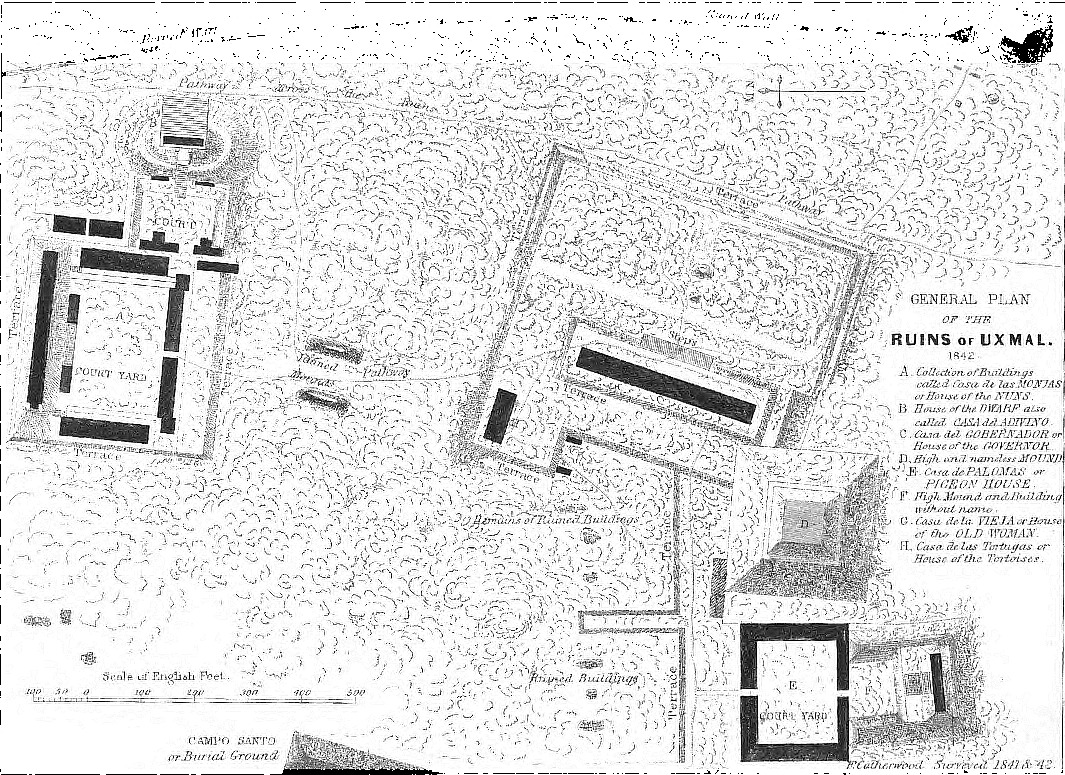
\includegraphics[width=\linewidth]{./media/images/if_cover}%
  \label{fig:if_cover}%                                                 
  \end{center}
\end{figure*}
\smallbreak
\noindent \textbf{\large{\emph{Incidents of Travel in Yucatan}}}
\smallbreak
\noindent Passing through the arched gateway, we enter a noble courtyard, with four great façades looking down upon it, each ornamented from one end to the other with the richest and most intricate carving known in the art of the builders of Uxmal; presenting a scene of strange magnificence, surpassing any that is now to be seen among its rains. This courtyard is two hundred and fourteen feet wide, and two hundred and fifty-eight feet deep. At the time of our first entrance it was overgrown with bushes and grass, quails started up from under our feet, and, with a whirring flight, passed over the tops of the buildings. Whenever we went to it, we started flocks of these birds, and throughout the whole of our residence at Uxmal they were the only disturbers of its silence and desolation. 
\smallbreak
\noindent \textbf{\emph{Courtyard Entrance}}
\smallbreak
\noindent Among my many causes of regret for the small scale on which I am obliged to present these drawings, none is stronger than the consequent inability to present, with all their detail of ornament, the four great façades fronting this courtyard. There is but one alleviating circumstance; which is, that the side most richly ornamented is so ruined that, under any circumstances, it could not be presented entire.
\smallbreak
\noindent \textbf{\emph{>ne}}
\smallbreak
\noindent \textbf{\emph{Southeast Façade}}
\smallbreak
\noindent This façade is on the left of the visiter entering the courtyard. It is one hundred and seventy-three feet long, and is distinguished by two colossal serpents entwined, running through and encompassing nearly all the ornaments throughout its whole length. The two plates which follow represent the only parts remaining.
\smallbreak
\noindent \textbf{\emph{>}}
% \subsection{creating a base tads3 system}
\subsection{pull tads3 javascript extension}
The ability to write inline Javascript into \textsc{tads3} code is handled by
Ben Cressey's excellent webscrptres
extension.\marginnote{\href{https://bitbucket.org/bcressey/t3ext}{Ben Cressey's
    webscrptres extension}} The extension may by dowloaded as a compressed
archive or may be 'pulled' from the source repository. The repository may be
pulled either to your local project directory
(\texttt{/home/cstevens/doc/gps/lib} in this case) or globally. This example
installs Cressey's extensions globally as it is convenient for future builds.
You will have to remember to re\textendash pull the extension for each new work
you create. Localized extensions, however, prevents potential versioning
problems and keeps your projects self\textendash contained:
\begin{lstlisting}
  cd /usr/local/share/frobtads/tads3/lib
  sudo sudo git clone https://bitbucket.org/bcressey/t3ext.git 
\end{lstlisting}
The repository will now be cloned to
\begin{lstlisting}
/usr/local/share/frobtads/tads3/lib/t3ext
\end{lstlisting}
\subsection{modify Makefile-web.t3m}
Make sure \texttt{\scriptsize{adv3/adv3web}} is defined prior to
\texttt{\scriptsize{t3ext/webui/webscript}} to avoid webscript's ``initDisplay''
object being loaded before \textsc{tads3}'s base \textsc{adv3web}. The compiler
will issue an error to this effect if the base library is not loaded before the
\textsc{webscript} library is loaded. Here is
\texttt{\scriptsize{Makefile-web.t3m}} in it's entirety:
\begin{lstlisting}
# Standard TADS comments above
# This project was generated using Anthony Irwin's Yeoman Generator
# generator-tads you can get the latest version from
# https://github.com/anthonyirwin82/generator-tads

# To compile the web version run t3make -f Makefile-web

# To test the web version run the following command:
# frob -i plain -s 44 -N 00 -p gps-web.t3

-we
-D TADS_INCLUDE_NET
-D LANGUAGE=en_us
-D MESSAGESTYLE=neu
-Fy obj
-Fo obj
-v
-o gps-web.t3

##sources
-lib system
-lib webui
-lib adv3/adv3web
# javascript hook
-lib t3ext/webui/webscript

-source tadsnet
-source gps

## rooms
-source src/rooms/se_facade/se_facade

## gps daemon
-source lib/gps_daemon.t

-res
GameInfo.txt
\end{lstlisting}
\section{enabling gps}
\begin{itemize}[leftmargin=0em]
\item From your base directory (\texttt{\scriptsize{/home/cstevens/doc/gps}} in this case), create a '\texttt{lib}'
(*nix parlance for supporting libraries) directory
\begin{lstlisting}
  mkdir /home/cstevens/lib/
\end{lstlisting}
\item Create a file called \texttt{\scriptsize{gps\_daemon.t}} under the \texttt{lib} directory with the contents listed below. This code contains the correct
  \textsc{gps} coordinates for our two locations and the system should thus
  compile. We'll review how to find and test the coordinates in the
  \emph{Finding GPS Coordinates} section on page \pageref{sec:coordinates} and
  the \emph{Testing} section on page \pageref{sec:testing}.
  \marginnote{GPS daemon code for passing client\textendash browser GPS
    information to \textsc{tads3}}[2em]
\begin{lstlisting}
#charset "utf-8"
#include <adv3.h>
#include <en_us.h>
#include <bignum.h>

DefineIAction(GPS);

VerbRule(GPS)
        'gps'
        :  GPSAction
        verbPhrase = 'script/scripting'
;

#define JS(STR, ARGS...) JavaScript.eval( ## #@STR ##, ##ARGS ## )
modify GPSAction
    execAction()
{
        JS({

var options = {
    enableHighAccuracy: true,
    timeout: 5000,
    maximumAge: 30000 
};

function success(pos) {
    serverRequest("/webui/gpsEvent?lat=" + pos.coords.latitude
        + '&lon=' + pos.coords.longitude + '&acc=' + pos.coords.accuracy);
    console.log('lattitude: ' + pos.coords.latitude + ' longitude: ' + pos.coords.longitude + ' Accuracy: ' + pos.coords.accuracy);
};

function error(err) {
    console.warn('ERROR(' + err.code + '): ' + err.message);
};

navigator.geolocation.watchPosition(success, error, options);

        });
    }
;

// This is TADS3 Code
gpsEvent: WebResource
    vpath = '/webui/gpsEvent'

    processRequest(req, query)
    {
            /* Do something... */
            //note the limiting place number to 'loosen' range in lat/lon
            local latitude = new BigNumber('<<query['lat']>>',7);
            local longitude = new BigNumber('<<query['lon']>>',7);
            //turn the lat & lon into a string for case statement below
            local location = toString([latitude,longitude]);
            "<p>location: <<location>>   lat: <<latitude>>  lon: <<longitude>></p>";

            // switch(latitude,longitude)
            switch(location)
            {
              /* Courtyard Entrance */
            case ('20.3608,-89.7707'):
              if (me.isIn(firstRoom) == nil)
                {
                  me.scriptedTravelTo(firstRoom); 
                  /* send a new prompt */
                  commandWin.write('<br />&gt; '); 
                  commandWin.flushWin();

                  /* set the UI state */
                  commandWin.mode = 'inputLine';
                  commandWin.isInputOpen = true;

                  /* send the inputLine event to the client */
                  commandWin.sendWinEvent('<inputLine/>');
                } //end me.location
            break;
              /* Southeast Facade */
              case ('20.3612,-89.7709'): 
              if (me.isIn(se_facade) == nil)
                {
                me.scriptedTravelTo(se_facade);
                /* send a new prompt */
                commandWin.write('<br />&gt; '); 
                commandWin.flushWin();

                /* set the UI state */
                commandWin.mode = 'inputLine';
                commandWin.isInputOpen = true;

                /* send the inputLine event to the client */
                commandWin.sendWinEvent('<inputLine/>');
                } //end me.location
              break;
            default:
             {
                /* set the UI state */
                commandWin.mode = 'inputLine';
                commandWin.isInputOpen = true;

                /* send the inputLine event to the client */
                commandWin.sendWinEvent('<inputLine/>');

             }
         }
        sendAck(req);
    }
;
\end{lstlisting}
\end{itemize}
Notice that the \textsc{gps} daemon code is actually written in \textsc{tads3}
with embedded Javascript. After the header include statements we'll define a new
\textsc{tads3} verb called \texttt{gps}.
\begin{lstlisting}
DefineIAction(GPS);

VerbRule(GPS)
        'gps'
        :  GPSAction
        verbPhrase = 'script/scripting'
;
\end{lstlisting}
The next line tells \textsc{tads3} that anytime it sees the \texttt{\scriptsize{JS()}}
directive that it should be passed to the browser for direct processing. The
power here lies in the ability for the directive to pass variables
back\textendash and\textendash forth to the \textsc{tads3} compiler.
\begin{lstlisting}
#define JS(STR, ARGS...) JavaScript.eval(## #@STR ##, ##ARGS ##)
\end{lstlisting}
The \texttt{\scriptsize{modify GPSAction}} defines the action that should be taken when the
\texttt{gps} command is executed. In this case the command initiates the
browser's client\textendash side \textsc{gps} subsystem with the Javascript code that
immediately follows, ie., the statements enclosed in the \texttt{\scriptsize{JS\{(...)\}}} directive.

The actual accumulation of the Interlocutor's position is collected via the
sparsely named \texttt{lat} and \texttt{lon} variables. The command also
provides an accuracy variable (\texttt{acc}) that you may use for testing or as
a part of an expanded subroutine to ensure that your positional data is correct.
\marginnote{The polling loop queries the Interlocutor's \textsc{gps} device
  every five seconds producing position variables for processing}[2em]
\begin{lstlisting}
    serverRequest("/webui/gpsEvent?lat=" + pos.coords.latitude
        + '&lon=' + pos.coords.longitude + '&acc=' + pos.coords.accuracy);
\end{lstlisting}
Amazingly we return to \textsc{tads3} code where the \textsc{javascript} \textsc{lat/lon}
variables are passed as an array for assignment back into \textsc{tads3}
\begin{lstlisting}
 local latitude = new BigNumber('<<query['lat']>>',7);
 local longitude = new BigNumber('<<query['lon']>>',7);
\end{lstlisting}
The \texttt{\scriptsize{latitude}} and \texttt{\scriptsize{longitude}} numbers are cut to give a slightly
wider range of positions (within 10 meters or so) accepted to create an event
that the Interlocutor has actually entered the area of interest. The variables
are now converted into a text string for testing by a \texttt{\scriptsize{case}} statement
later on and a print statement is added for use during development.
\begin{lstlisting}
local location = toString([latitude,longitude]);
"<p>location: <<location>>   lat: <<latitude>>  lon: <<longitude>>
</p>";
\end{lstlisting}
Once matching pair of coordinates are received a \textsc{tads3} \texttt{\scriptsize{me.scriptedTravelTo}} event is triggered.
\begin{lstlisting}
/* Southeast Facade */
case ('20.3612,-89.7709'): 
  if (me.isIn(se_facade) == nil)
  {
    me.scriptedTravelTo(se_facade);
  ...
\end{lstlisting}
\marginnote{\href{http://www.tads.org/howto/t3npcTravel.htm}{scriptedTravelTo
    details from the \textsc{tads3} Howto guide}}[1em]
Notice that a \emph{scripted} event is triggered. The \texttt{\scriptsize{scriptedTravelTo()}} method
always carries out a single nested action, which means that it does everything
that would normally happen when the Interlocutor moves into this location. This
includes any narration, travel connector descriptions, tripped events beyond
location, etc. An exciting possibility that immediately comes to mind is a work
where a 'bonus' location isn't overtly stated; one that is only inferred by clues
found elsewhere. When the Interlocutor approaches the 'secret' location an
entire story line opens up.
\marginnote{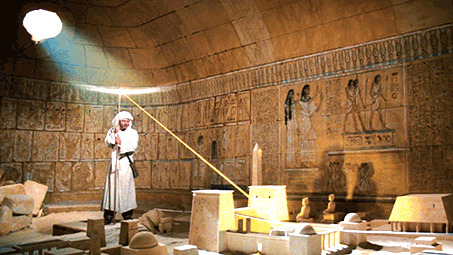
\includegraphics[width=\linewidth]{./media/images/indie}%
  \label{fig:indie}\\ Locations inferred only through clues found elsewhere
}[-6em]
Finally, these lines perform some house cleaning after the location change by
resetting the \textsc{ui} state and preparing the parser for input.
\begin{lstlisting}
/* set the UI state */
commandWin.mode = 'inputLine';
commandWin.isInputOpen = true;

/* send the inputLine event to the client */
commandWin.sendWinEvent('<inputLine/>');
\end{lstlisting}
\subsection{finding gps coordinates}
  \label{sec:coordinates}%                                                 
\begin{figure*}[h]                                                           
 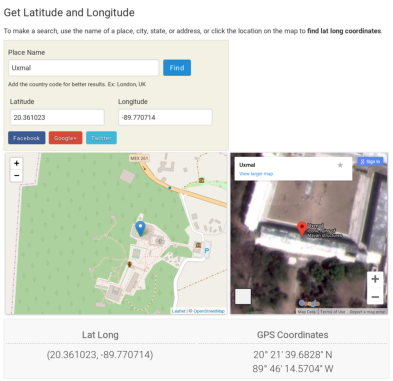
\includegraphics[width=\linewidth]{./media/images/lat_lon.pdf}%
  \scriptsize{\textsc{\\Getting Latitude and Longitude coordinates} is
    straight\textendash forward using \textsc{latlon.net}.}
  \label{fig:lat_lon}%                                                 
\end{figure*}
\begin{figure*}[h]                                                           
 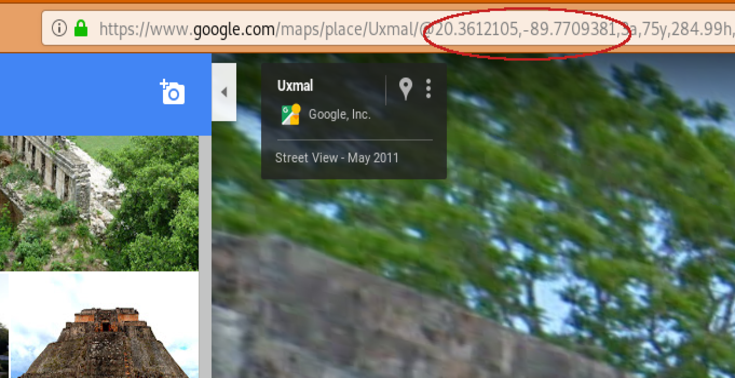
\includegraphics[width=\linewidth]{./media/images/url.pdf}%
  \scriptsize{\textsc{\\Reading the lat/lon} coordinates from Google maps}
  \label{fig:facade}%                                                 
\end{figure*}
\marginnote{\href{https://www.latlong.net/}{latlong.net gives geographic
    coordinate information through a Google Maps interface}}
\noindent At least two methods exist for zeroing in your \textsc{if} geography's
\textsc{gps} coordinates. The first is through \textsc{latlong.net}; the second
involves reading the \textsc{url} line from Google Maps. \textsc{latlong.net} provides a map and satellite view opposite each other. The coordinates you need
for entry into the \textsc{if gps} system are listed below on the left hand
side. Once you've established your initial position you can use Google Maps
street view to each position and quickly read off the lat/lon entries in your
current position's \textsc{url} status line.
\begin{figure*}[h]                                                           
 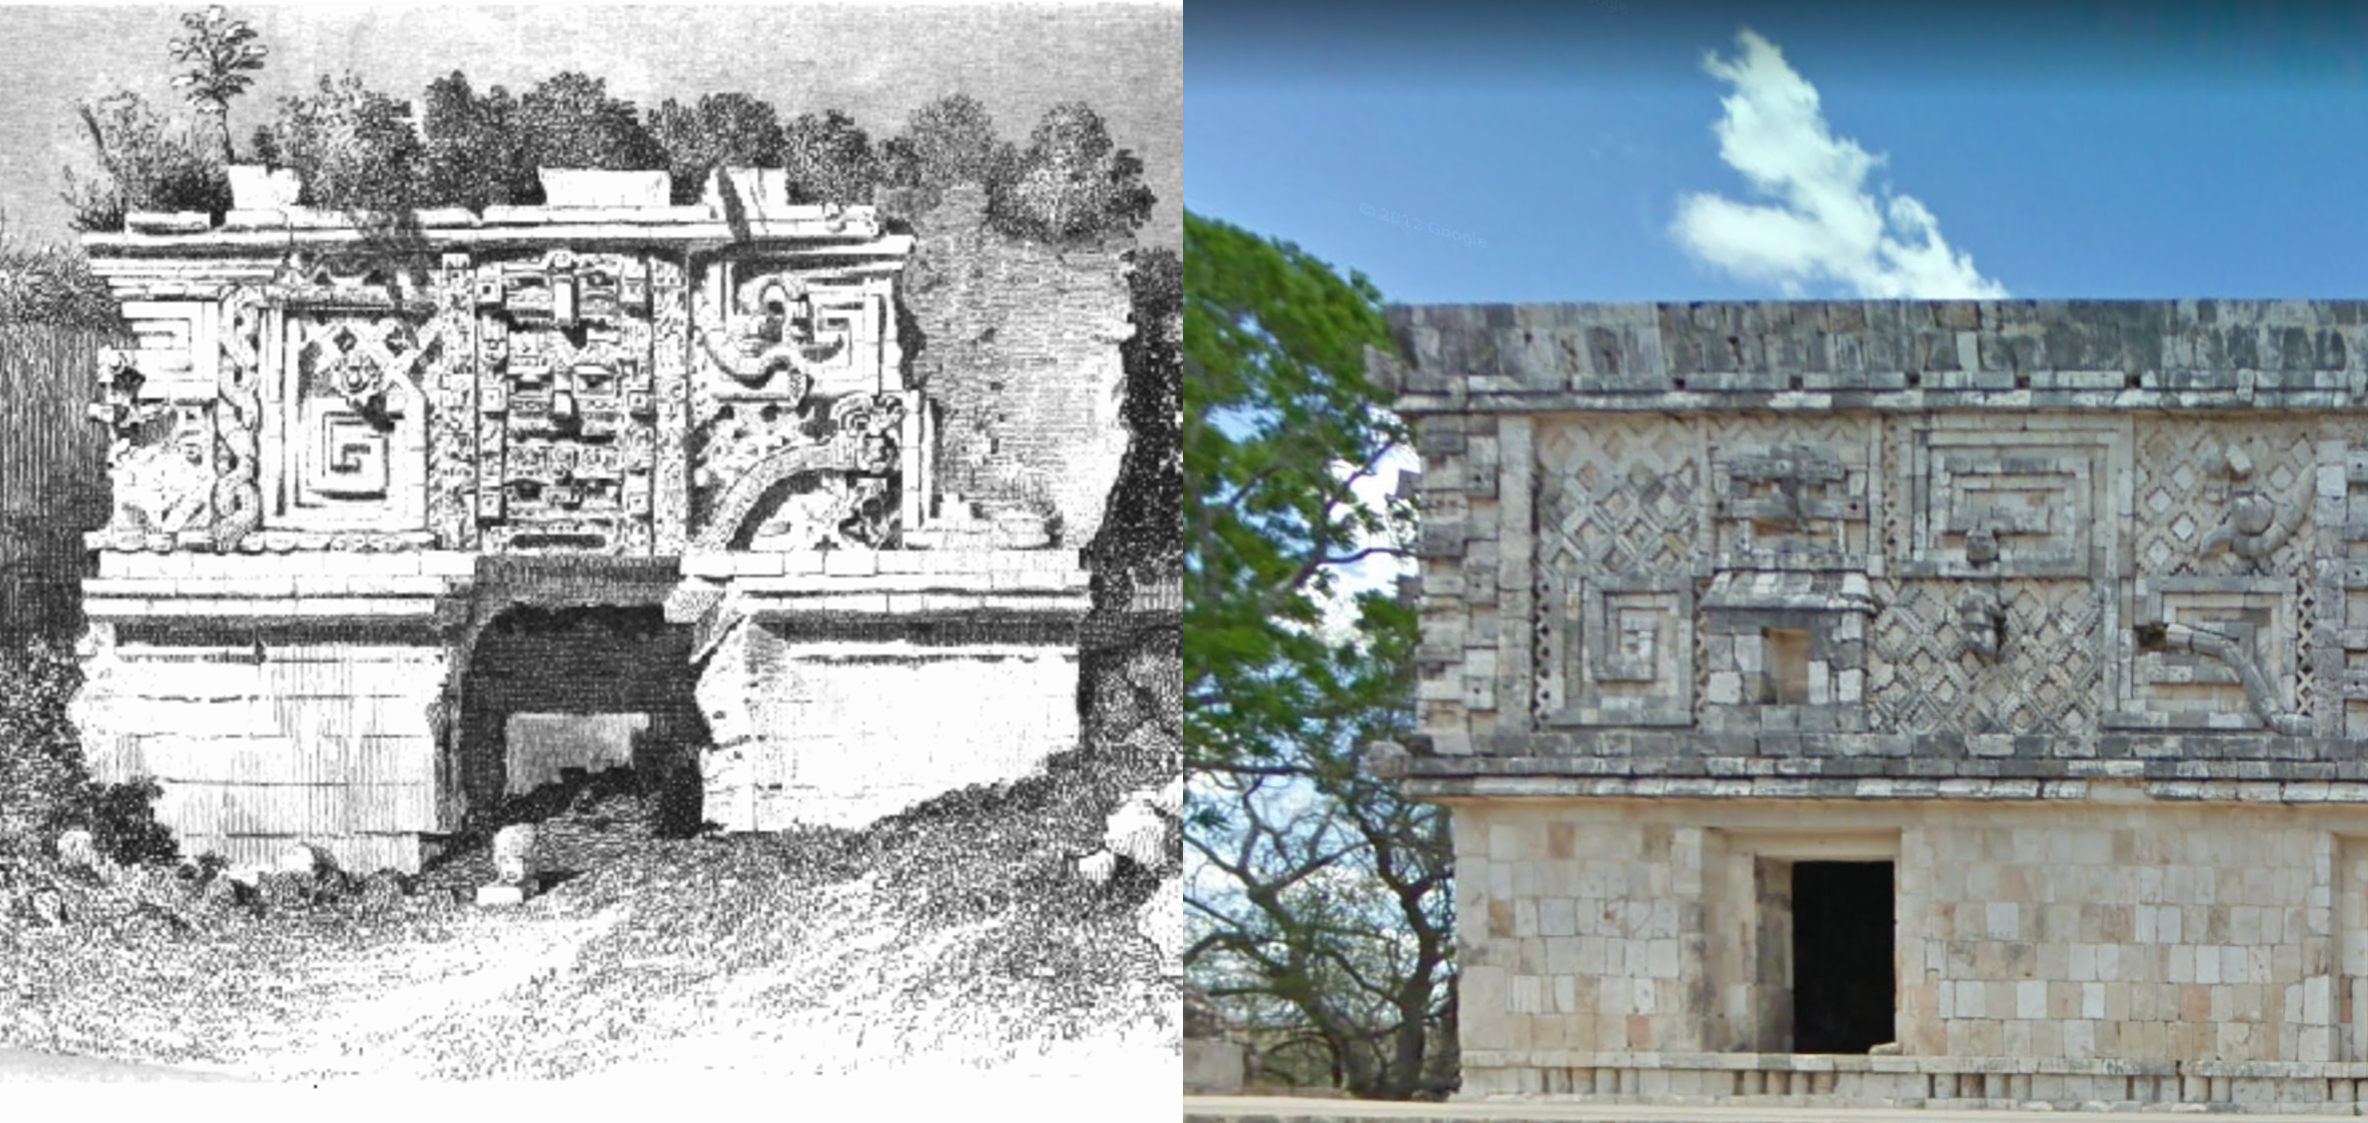
\includegraphics[width=\linewidth]{./media/images/court_facade.pdf}%
  \scriptsize{\textsc{\\Façade of the Monjas sketch} from \emph{circa} 1848 shown beside the Façade today}
  \label{fig:facade}%                                                 
\end{figure*}
\section{testing}
\label{sec:testing}
Once you've compiled your draft \textsc{if} with each area's respective \textsc{gps}
coordinates you'll need to test each location to ensure that the system works
when the browser sends a pair of coordinates that match one of your designated
sites. This is achieved using the browser's \textsc{about:config} options to
manually change the browser's reported latitude and longitude coordinates. Once
the browser is set up to modify it's coordinate reporting testing your testing
is mostly a matter of organization to ensure that each position is checked for
accuracy and completeness.

\marginnote{\href{https://www.comparitech.com/blog/vpn-privacy/change-location-chrome-firefox-spoof/}{Detailed description for changing your browser's reported position using the browser's \textsc{about:config conf} configuration parameters}}
Several browser plugins exist to ``spoof'' your browser's reported position. No
plugin I've tested to date works correctly; even though the coordinates appear
to be modified by the plugin the system at the reporting level the \textsc{Javascript}
code pulls from the \textsc{gps} coordinates of your location's nearest central
office \textsc{(co)} location.

Testing involves the following steps:
\begin{itemize}[leftmargin=0em]
  \item{Modify the browser's configuration to point to the location you wish to
      test}
  \item{Compile and run your \textsc{if}prototype}
    \end{itemize}
\begin{itemize}[leftmargin=0em]
\item{Open a new tab in your browser and type the command \texttt{\scriptsize{about:config}}
    in your browser and agree that you understand that manually changing the
    configuration ``may void your warranty''}
\item{Search for the \texttt{geo.wifi.uri} parameter}
  \item{modify the \textsc{json} object to the coordinates listed in an
      adjacent area in the prototype (the \texttt{\scriptsize{se\_facade}}
      located at \texttt{\scriptsize{lat 20.3612 lon -89.7709}} in this case)}
\end{itemize}
  \begin{lstlisting}
    data:application/json,{"location": {"lat": 20.3612, "lng": -89.7709}, "accuracy": 1.0}
  \end{lstlisting}
\begin{figure*}[h]                                                           
 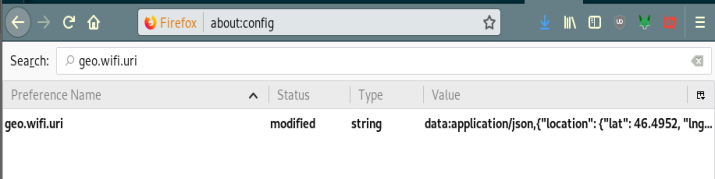
\includegraphics[width=\linewidth]{./media/images/gps_config.pdf}%
  \scriptsize{\textsc{\\Using the browser's geo.enabled} parameter in the
    browser configuration dialog ()}
  \label{fig:about_config}%                                                 
\end{figure*}
\subsection{compiling and running your prototype}
\begin{itemize}[leftmargin=0em]
\item{compile your \textsc{if} prototype with the \textsc{t3make} command}
\begin{lstlisting}
t3make -a -f Makefile-web.t3m
\end{lstlisting}
\item{Next, run the \textsc{frobtads} interpreter and click the resulting link}
\begin{lstlisting}
frob -i plain -s 44 -N 00 -p gps-web.t3

connectWebUI:http://localhost:40241/?TADS_session=680c40b7-bd92-04e6-297af4b44661-61c2
\end{lstlisting}
\item{Enter the \texttt{gps} command at your \textsc{if} instance's parser command prompt to initiate the \textsc{gps} daemon}
\begin{lstlisting}
  gps
\end{lstlisting}
\item{Permit the browser to access your location from the browser's pop\textendash up dialog box.}
\end{itemize}
You should now see the location service working anytime you execute a parser
command. The environment looks similiar to this (the Courtyard Entrance description is truncated):
\begin{quote}
  \textbf{\emph{Courtyard Entrance}}
  
Among my many causes of regret for the small scale on which I am obliged to
present these drawings, none is stronger than the consequent inability to
present, with all their detail of ornament, the four great façades fronting this
courtyard.
\smallskip

\textbf{\emph{>gps}}
\smallskip

Nothing obvious happens.
\smallskip

\textbf{\emph{>look}}
\smallskip

location: 46.4952,-124.0508 lat: 46.4952 lon: -124.0508 
\end{quote}
The location as a string along with the \texttt{lat} and \texttt{lon} variables
are printed for debugging. This may be changed for production by commenting out
the following lines in \texttt{\scriptsize{gps\_daemon.t}}.

\begin{lstlisting}
"<p>location: <<location>>   lat: <<latitude>>  lon: <<longitude>></p>";
\end{lstlisting}
After a few moments you should see your location change; you may need to refresh
your browser depending on your browser's settings and enabled plugins. 
\begin{figure*}[h]                                                           
\hspace*{-1.75cm} 
 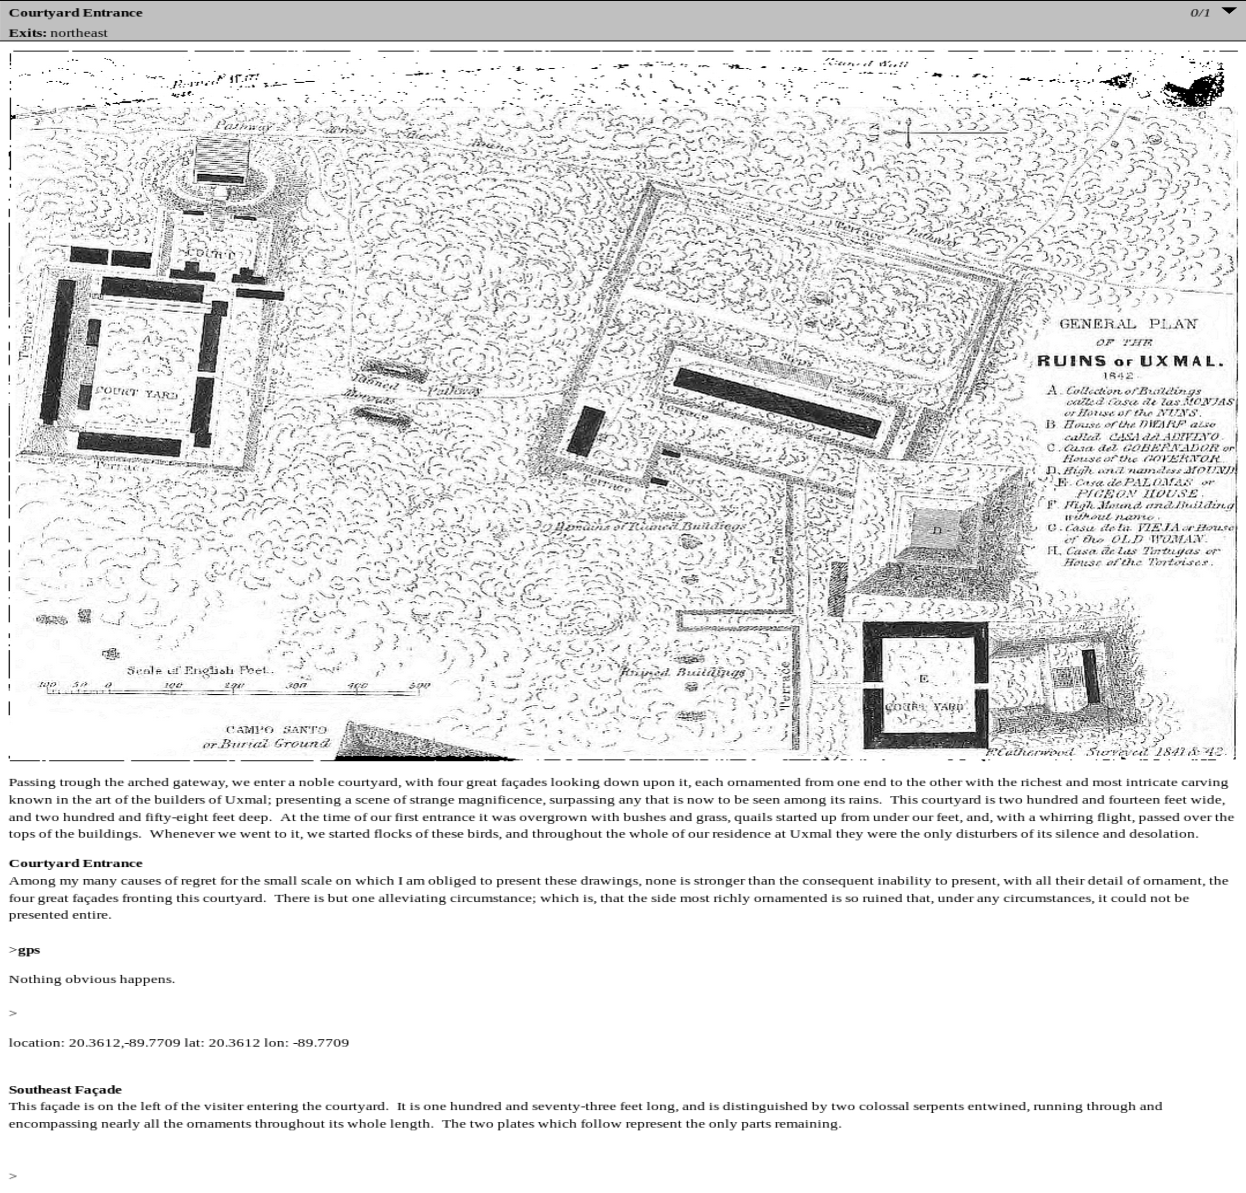
\includegraphics[width=0.9\paperwidth]{./media/images/switch.pdf}%
  \scriptsize{\textsc{\\Finished product depicting} the triggered site change
    when the browser reports coordinates matching the work's location}
  \label{fig:switched}%                                                 
\end{figure*}

% * Testing: spoof geo in browser
%   ** geo-spoofing plugins do not work.
%   ** Changing geo point in browser:
% https://www.comparitech.com/blog/vpn-privacy/change-location-chrome-firefox-spoof/
%This is a test ov figuring out why this thing is so weird.

% * Also need to refresh the page after testing.
% \reversemarginpar\marginnote{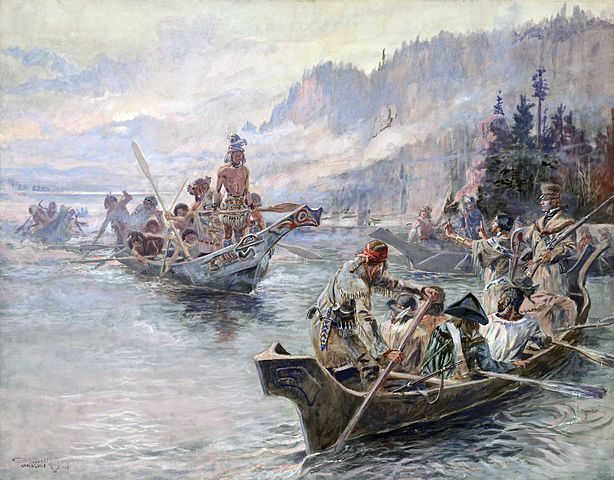
\includegraphics[width=\linewidth]{./media/images/lewis}\href{https://www.youtube.com/watch?v=NJarxpYyoFI}{\\This is the marginnote caption(linked)}}
